\documentclass{ieeeojies}
\usepackage{cite}
\usepackage{amsmath,amssymb,amsfonts}
\usepackage{algorithmic}
\usepackage{graphicx}
\usepackage{textcomp}
\usepackage{array}
\usepackage[table]{xcolor}
\usepackage{multirow}
\usepackage{multicol}
\usepackage{float}
\usepackage[T1]{fontenc}
\def\BibTeX{{\rm B\kern-.05em{\sc i\kern-.025em b}\kern-.08em
    T\kern-.1667em\lower.7ex\hbox{E}\kern-.125emX}}

\begin{document}
\title{FFT, TimesNet, and Random Forest in Real Estate Stock Market Analysis}

\author{\uppercase{Phan Chi Cuong}\authorrefmark{1},
\uppercase{Nguyen Le Khang\authorrefmark{2}, and Le Pham Quoc Bao}\authorrefmark{3}}

\address[1]{Faculty of Information Systems, University of Information Technology, (e-mail: 21520673@gm.uit.edu.vn)}
\address[2]{Faculty of Information Systems, University of Information Technology, (e-mail: 21520960@gm.uit.edu.vn)}
\address[3]{Faculty of Information Systems, University of Information Technology, (e-mail: 21521849@gm.uit.edu.vn)}

\markboth
{Author \headeretal: Phan Chi Cuong, Nguyen Le Khang, Le Pham Quoc Bao}
{Author \headeretal: Phan Chi Cuong, Nguyen Le Khang, Le Pham Quoc Bao}

\begin{abstract}
  This study investigates the effectiveness of Fast Fourier Transform (FFT), Time Series Network (TimeSNet), and Random Forest (RF) models in predicting stock prices within the Vietnamese real estate market.  We apply these models independently to historical daily closing prices of three major real estate companies from 2019 to 2024, exploring how each method contributes to understanding and forecasting stock price movements. FFT is utilized to reveal underlying periodic patterns, TimeSNet to capture temporal dependencies, and RF to provide robust predictions. The results offer insights into the strengths and weaknesses of each model for this specific market, providing valuable information for investors and policymakers.
\end{abstract}

\begin{keywords}
  Placeholder
\end{keywords}

\titlepgskip=-15pt

\maketitle

\section{Introduction}
\label{sec:introduction}
Time-series forecasting plays a crucial role in decision-making across various domains. Its significance lies in its ability to provide valuable insights into future trends and patterns in time-dependent data. For instance, accurate predictions of stock prices, interest rates, and foreign exchange rates are essential for informed investment decisions in finance. Similarly, healthcare organizations rely on forecasting patient demand and resource utilization to allocate resources effectively and improve patient care. Energy management companies use time series forecasting to optimize energy production, distribution, and consumption. The accuracy and efficiency of time-series forecasting models significantly impact organizational performance and decision-making processes.

In this paper, we explore an innovative approach to enhance time-series forecasting using the Fast Fourier Transform (FFT). The FFT algorithm extracts frequency-domain features from time series data, offering a promising avenue for improving forecast accuracy and computational efficiency. Our investigation involves a comparative analysis of models trained with FFT-based features against traditional time domain features. We apply this approach to predict stock prices of real estate companies, leveraging not only FFT but also other techniques such as TimesNet and Random Forest. Through our study, we shed light on the interpretability of frequency domain features and their relationship with underlying time series patterns, emphasizing the potential of FFT-based feature engineering in enhancing forecasting models.

\section{Related Works}

In recent years, many stock prediction models have been researched and many articles have been published, such as: \\

Hind Daori, Alanoud Alanazi, Manar Alharthi, Ghaida Alzahrani (2022)\cite{b1} used Artificial Neural Network (ANN), Random Forest
Classifier, Logistic Regression,and then analyze and predict the
patterns of previous stock prices and the results showed that the models were efficient and produced better results.\\

Hugo Souto(2023) \cite{b2} has researched about TimesNet for Realized Volatility Prediction. Finally, they concluded that TimesNet stands out as a reliable and effective benchmark model for researching realized volatility. Although it may not always surpass NBEATSx and NHITS in every metric, its strong performance and consistency make it a valuable option, especially when compared to TFT. Overall, TimesNet presents a balanced and dependable choice that combines reliability with effectiveness, making it a suitable neural network model for researchers and practitioners in the field of realized volatility. \\

In another article by Bohumil Stádník, Jurgita Raudeliuniene, Vida Davidavičienė \cite{b3}, they pointed out that the Fourier analysis may not be advantageous for investors forecasting stock market prices as it fails to detect existing predominant cycles. An attempt to identify significant periods in the US stock market data using FFT, a method of Fourier analysis, proved to be unacceptable. Similar failures can be expected with other liquid investment instruments or financial data series. Despite this, Fourier analysis is still used for forecasting in finance and its benefits are a topic of discussion among financial market practitioners and academicians.


\section{Materials}
Placeholder line
\subsection{Dataset}

The dataset comprises historical daily closing stock prices (in Vietnamese Dong - VND) for three prominent Vietnamese real estate companies:
 \\
  \indent\textbullet\ Quoc Cuong Gia Lai Joint Stock Company (QCG) \\
  \indent\textbullet\ Dat Xanh Group Joint Stock Company (DXG) \\
  \indent\textbullet\ Vinhomes Joint Stock Company (VHM) \\
  \\
The data spans a five-year period from March 1, 2019, to March 1, 2024.  While the raw data includes additional attributes such as opening price, high, low, volume, and change, this study focuses solely on the "Close" price to develop predictive models for future closing price movements.

\subsection{Descriptive Statistics}
\begin{table}[H]
  \centering
  \caption{QCG, VHM, DXG’s Descriptive Statistics}
\begin{tabular}{|>{\columncolor{red!20}}c|c|c|c|}
    \hline
     \rowcolor{red!20} & DXG & VHM & QCG \\ \hline
     Observations & 0 & 0 & 1252 \\ \hline
     Mean & 0 & 0 & 7586.17\\ \hline
     Median & 0 & 0 & 7105\\ \hline
     Std & 0 & 0 & 3102.55\\ \hline
     Min & 0 & 0 & 3320\\ \hline
     Max & 0 & 0 & 23200\\ \hline
     25\% & 0 & 0 & 4960\\ \hline
     50\% & 0 & 0 & 7105\\ \hline
     75\% & 0 & 0 & 9182.5\\ \hline
    Skewness & 0 & 0 & 1.13\\ \hline
    Kurtosis & 0 & 0 & 1.68\\ \hline

     
\end{tabular}
\end{table}
\begin{figure}[H]
  \centering
  \begin{minipage}{0.23\textwidth}
  \centering
  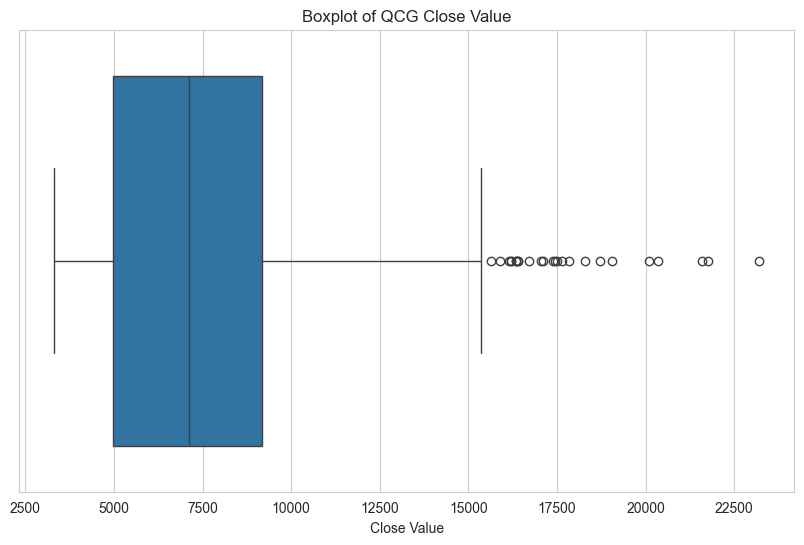
\includegraphics[width=1\textwidth]{bibliography/Figure/QCGboxplot.png}
  \caption{QCG stock price's boxplot}
  \label{fig:1}
  \end{minipage}
  \hfill
  \begin{minipage}{0.23\textwidth}
  \centering
  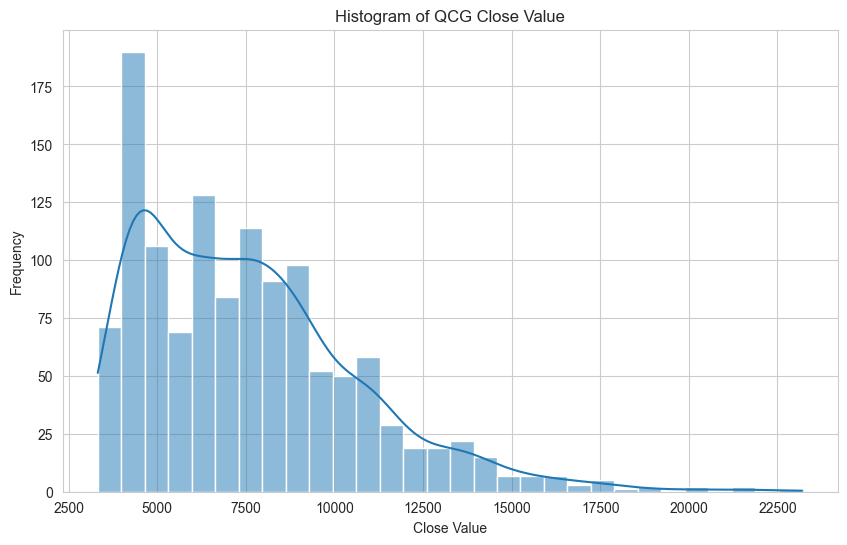
\includegraphics[width=1\textwidth]{bibliography/Figure/QCGhist.png}
  \caption{QCG stock price's histogram}
  \label{fig:2}
  \end{minipage}
\end{figure}


\section{Methodology}
Placeholder line
\subsection{Linear Regression}
Placeholder
\[Y=\beta_0+\beta_1X_1+\beta_2X_2+\cdots+\beta_kX_k+\varepsilon\]
Where:\\
	\indent\textbullet\ Y is the dependent variable (Target Variable).\\
	\indent\textbullet\ \(X_1, X_2, \ldots, X_k\) are the independent (explanatory) variables.\\
	\indent\textbullet\ \(\beta_0\) is the intercept term.\\
	\indent\textbullet\ \(\beta_1,..., \beta_k\) are the regression coefficients for the independent variables.\\
	\indent\textbullet\ \(\varepsilon\) is the error term.
 

\section{Result}
Placeholder line
\subsection{Evaluation Methods}
\textbf{Mean Percentage Absolute Error} (MAPE): is the average percentage error in a set of predicted values.\\
\[MAPE=\frac{100\%}{n}  \sum_{i=1}^{n} |y_i-\hat{y_i} |  = 1 \]\\
\textbf{Root Mean Squared Error} (RMSE): is the square root of average value of squared error in a set of predicted values.\\
\[RMSE=\sqrt{\sum_{i=1}^{n} \frac{(\hat{y_i}-y_i )^2}{n} }\]\\
\textbf{Mean Absolute Error} (MSLE):is the relative difference between the log-transformed actual and predicted values.\\
\[MSLE=\frac{1}{n}\sum_{i=1}^{n}(log(1+\hat{y_i})-log(log(1+y_i))^2\]
Where: \\
	\indent\textbullet\ \(n\) is the number of observations in the dataset.\\
	\indent\textbullet\ \(y_i\)  is the true value.\\
	\indent\textbullet\ \(\hat{y_i}\) is the predicted value.
\subsection{DXG Dataset} 
\begin{table}[H]
    \centering
    \begin{tabular}{|c|c|c|c|c|}
         
    \end{tabular}
    \caption{DXG Dataset's Evaluation}
    \label{vcbresult}
\end{table}

\subsection{VHM dataset} 



\subsection{QCG dataset} 

\section{Conclusion}
 Placeholder line
\subsection{Summary}
Placeholder
\subsection{Future Considerations}
Placeholder line
\section*{Acknowledgment}
\addcontentsline{toc}{section}{Acknowledgment}
Placeholder line

%% UNCOMMENT these lines below (and remove the 2 commands above) if you want to embed the bibliografy.
\begin{thebibliography}{00}
\bibitem{b1} Hind Daori, Alanoud Alanazi, Manar Alharthi, Ghaida Alzahrani
 ,  ''Predicting Stock Prices Using the Random ForestClassifier'', November, 14th, 2022.
\bibitem{b2} Hugo Souto, 2023, ''TimesNet for Realized Volatility Prediction
''.
\bibitem{b3} Bohumil Stádník, Jurgita Raudeliuniene, Vida Davidavičienė , 2016. Fourier Analysis For Stock Price Forecasting: Assumption And Evidence .

\end{thebibliography}
%%%%%%%%%%%%%%%


\EOD

\end{document}
